\documentclass[11pt, a4paper, twoside, openright]{article}
\usepackage{import}
\usepackage[english]{babel}
\usepackage[T1]{fontenc}
\usepackage{textcomp}
\usepackage[utf8]{inputenc}
\usepackage{graphicx}
\usepackage{amsmath}
\usepackage{amsfonts}
\usepackage{picture}
\usepackage[parfill]{parskip}
\usepackage[top=1in, bottom=1in, left=1.25in, right=1.25in]{geometry}
\usepackage{amssymb}
\usepackage{amsthm}
\usepackage{ccaption}
\usepackage{tikz}
\usetikzlibrary{matrix}

\DeclareMathOperator{\id}{id}
\DeclareMathOperator{\argmin}{argmin}
\DeclareMathOperator{\tr}{tr}
\DeclareMathOperator{\err}{err}
\DeclareMathOperator{\Err}{Err}
\DeclareMathOperator{\ave}{ave}
\DeclareMathOperator{\corr}{corr}

%\theoremstyle{plain}
% \renewcommand{\thesection}{\arabic{chapter}.\arabic{section}}
% \newtheorem{thm}{Theorem}[chapter]
% \newtheorem{lemma}[thm]{Lemma}
% \newtheorem{definition}[thm]{Definition}
% \newtheorem{example}[thm]{example}
% \newtheorem{prop}[thm]{Proposition}
% \newtheorem{remark}[thm]{Remark}

\usepackage{subcaption}



% \setlength\bibitemsep{2\itemsep}

% \addbibresource{bibliography.bib}

% \DeclareNameAlias{default}{last-first}
% \usepackage[backend=bibtex]{bibtex}
%\bibliographystyle{plain}
%\bibliography{bibliography}
%\usepackage{natbib}
%\bibliographystyle{unsrt}
%\usepackage{cite}

%\usepackage{color}
% \usepackage{listings}
% \lstloadlanguages{R}
% \lstset{language=R, 
%         keywordstyle=[1]\color{black}\ttfamily,
%         %keywordstyle=[2]\color{green},        
%         commentstyle=\color{red},
%         %morekeywords={imp}
%         %keywordstyle=\color{Blue}
%         %classoffset=0
%         %keywordstyle={[1]\color{Blue}},
%         %keywordstyle=[2]\color{Purple},
%         %morekeywords=[1]{mean.imp},
%         %morekeywords=[2]{for, if}
% }

\usepackage[font=small]{caption}
%\usepackage{appendix}

\newcommand{\defeq}{\mathrel{\mathop:}=}
%\DeclareMathOperator{\dim}{dim}
\newenvironment{sistema}{\left\lbrace\begin{array}{@{}l@{}}}
{\end{array}\right.}


\begin{document}
\section{Dataset}
$86$ subjects, mean age $144.1$ ($\sim 12$ years), sd $30.90$.
\begin{figure}[h!] 
\centering
\includegraphics[width=1\textwidth]{/media/data/dyslexia_project/plot/bw_age.pdf}
\caption{Age distribution.}
\label{fig:1}
\end{figure}

\textbf{Clinical profile:}\\
\begin{itemize}
\item DSM5: classification of dyslexia in `low' (class 1), `medium'
  (class 2), `high' (class 3).\\

\begin{table}[h!]
  \begin{center}
  \begin{tabular}{|c|c|}
    \hline
    DSM5 class & number of subjects\\
    \hline \hline
    class 1 & 42\\
    \hline
    class 2 & 14\\
    \hline
    class 3 & 30\\
    \hline
  \end{tabular}
\caption{Clinical profile. DSM5 classification.}
\label{tab:1}
\end{center}
\end{table}

\end{itemize}

\textbf{Cognitivie profile:}\\
\begin{itemize}
\item WISC-III/IV: 5 \emph{scores}, 7 \emph{subscales}.\\
  Only the subscale scores are considered. This in order to perform
  machine learning procedures without involving dependent variables.\\
  The subscale scores were reduced to 7 after the two instruments,
  WISC-III and WISC-IV, were merged.

  Subscale mean: $10$.\\
  Subscale standard deviation: $3$.
\begin{table}[h!]
\begin{center}
  \begin{tabular}{|c|c|c|c|}
    \hline
    WISC subscales & range & mean & sd\\
    \hline \hline
    dc & $6:18$&$11.13$&$2.86$\\
    \hline
    so & $4:17$&$10.36$&$2.79$\\
    \hline
    mc & $2:15$&$8.40$&$2.75$\\
    \hline
    cf & $1:14$&$7.60$&$2.67$\\
    \hline
    vc & $3:17$&$10.02$&$2.73$\\
    \hline
    co & $5:19$&$11.08$&$2.70$\\
    \hline
    rs & $2:16$&$9.36$&$2.88$\\
    \hline
  \end{tabular}
\end{center}
\caption{Cognitive profile. WISC subscales.}
\label{tab:2}
\end{table}

\begin{figure}[h!] 
\centering
\includegraphics[width=1\textwidth]{/media/data/dyslexia_project/plot/bw_wisc_no_out.pdf}
\caption{WISC subscale distribution.}
\label{fig:2}
\end{figure}

\begin{figure}[h!] 
\centering
\includegraphics[width=1\textwidth]{/media/data/dyslexia_project/plot/bw_wisc_no_out_class.pdf}
\caption{WISC subscale distribution by class.}
\label{fig:3}
\end{figure}

\clearpage

\item DDE: 4 \emph{scores} measuring word/non-word reading speed
  (wspeed, nwspeed) and accuracy (wacc, nwacc).\\
  DDE scores are sigma values, with $-2.0$ as the threshold for
  impairment. These values are computed with respect to age.
\begin{table}[h!]
\begin{center}
  \begin{tabular}{|c|c|c|c|}
    \hline
    DDE scores & range & mean & sd\\
    \hline \hline
    wspeed & $-13.43:-0.46$ & $-3.93$ & $2.61$\\
    \hline
    wacc & $-10.30:1.00$ & $-2.50$ & $2.40$\\
    \hline
    nwspeed & $-9.90:0.20$ & $-3.57$ & $2.24$\\
    \hline
    nwacc & $-9.00:1.30$ & $-1.33$ & $1.74$\\
    \hline
  \end{tabular}
\end{center}
\caption{Cognitive profile. DDE scores.}
\label{tab:3}
\end{table}

Outliers: subject 5, 673.\\
Subject 5 $\longrightarrow$ wspeed$=-13.43$, new range $-11.60:-0.46$\\
Subject 673 $\longrightarrow$ nwacc$=-9.00$, new range $-4.40:1.30$

\begin{figure}[h!] 
\centering
\includegraphics[width=1\textwidth]{/media/data/dyslexia_project/plot/bw_dde_no_out.pdf}
\caption{DDE score distribution.}
\label{fig:4}
\end{figure}

\begin{figure}[h!] 
\centering
\includegraphics[width=1\textwidth]{/media/data/dyslexia_project/plot/bw_dde_no_out_class.pdf}
\caption{DDE score distribution by class.}
\label{fig:5}
\end{figure}
\end{itemize}

\clearpage

In order to investigate the distribution of DSM5 classes and the
correlation between the scores we provide the graph below.
\begin{figure}[h!] 
\centering
\includegraphics[width=1\textwidth]{/media/data/dyslexia_project/plot/pairs_no_out.pdf}
\caption{Pair graph with DDE scores and WISC subscales. Correlation coefficient in the lower panel.}
\label{fig:6}
\end{figure}

\clearpage

\section{Data Analysis}
From previous Figures we can suppose that DSM5 classification can be
driven from DDE scores, hence DDE is a classifier, while WISC
subscales work as a modulator. We want to assess the following diagram
in order to provide a cognitive profile to the DSM5 classification (*).

\begin{center}
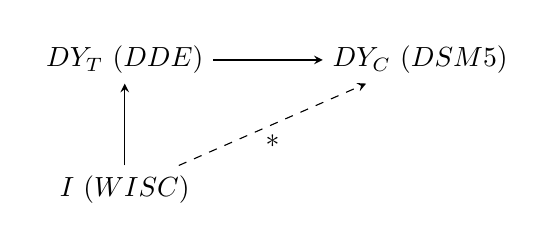
\begin{tikzpicture}
  \matrix (m) [matrix of math nodes,row sep=3em,column sep=4em,minimum width=2em]
  {
     DY_T\ (DDE) & DY_C\ (DSM5) \\
     I\ (WISC) & \\};
  \path[-stealth]
    (m-2-1) edge node [left] {} (m-1-1)
    (m-1-1) edge [left] node [below] {} (m-1-2)
    (m-2-1) edge [dashed] node [below] {*} (m-1-2);
\end{tikzpicture}
\end{center}

\small{$DY_T$: technical dyslexia, $DY_C$: clinical dyslexia, $I$: intelligence.}

\subsection{DDE scores}
Firstly we want to see if it is possible to reduce the number of DDE
variables, from 4 to 2, expressing the processing speed in function of
the processing accuracy.
\begin{figure}[h!] 
\centering 
\begin{subfigure}{1\textwidth}
\centering
\includegraphics[width=1\textwidth]{/media/data/dyslexia_project/plot/scat_ddew_no_out.pdf}
\caption{Scatterplot word accuracy against word speed in the three classes.}
\label{fig:7a}
\end{subfigure}
\end{figure}
\begin{figure}
\ContinuedFloat
\centering 
\begin{subfigure}{1\textwidth}
\centering
\includegraphics[width=1\textwidth]{/media/data/dyslexia_project/plot/scat_ddenw_no_out.pdf}
\caption{Scatterplot non-word accuracy against non-word speed in the three classes.}
\label{fig:7b}
\end{subfigure}
\caption{}
\label{fig:7}
\end{figure}

\clearpage

\subsection{WISC subscales}
We would like to parametrize the loess lines in
Figures~\ref{fig:7a}-\ref{fig:7b} in order to see if the variation of
WISC subscales determines a shift from the curve of one class to the
curve of another.\\
Let us now see how the WISC subscales vary according to the DDE
word/non-word speed scores. We highlight the first and third quantile,
along with the DSM5 classes.

\begin{figure}[h!] 
\centering 
\begin{subfigure}{1\textwidth}
\centering
\includegraphics[width=1\textwidth]{/media/data/dyslexia_project/plot/ws_dc.pdf}
\caption{}
\label{fig:8a}
\end{subfigure}
\end{figure}
\begin{figure}
\ContinuedFloat
\centering 
\begin{subfigure}{1\textwidth}
\centering
\includegraphics[width=1\textwidth]{/media/data/dyslexia_project/plot/nws_dc.pdf}
\caption{}
\label{fig:8b}
\end{subfigure}
\caption{Reading speed of words and non-words against subscale dc.}
\label{fig:8}
\end{figure}

\begin{figure}[h!] 
\centering 
\begin{subfigure}{1\textwidth}
\centering
\includegraphics[width=1\textwidth]{/media/data/dyslexia_project/plot/ws_so.pdf}
\caption{}
\label{fig:9a}
\end{subfigure}
\end{figure}
\begin{figure}
\ContinuedFloat
\centering 
\begin{subfigure}{1\textwidth}
\centering
\includegraphics[width=1\textwidth]{/media/data/dyslexia_project/plot/nws_so.pdf}
\caption{}
\label{fig:9b}
\end{subfigure}
\caption{Reading speed of words and non-words against subscale so.}
\label{fig:9}
\end{figure}

\begin{figure}[h!] 
\centering 
\begin{subfigure}{1\textwidth}
\centering
\includegraphics[width=1\textwidth]{/media/data/dyslexia_project/plot/ws_mc.pdf}
\caption{}
\label{fig:10a}
\end{subfigure}
\end{figure}
\begin{figure}
\ContinuedFloat
\centering 
\begin{subfigure}{1\textwidth}
\centering
\includegraphics[width=1\textwidth]{/media/data/dyslexia_project/plot/nws_mc.pdf}
\caption{}
\label{fig:10b}
\end{subfigure}
\caption{Reading speed of words and non-words against subscale mc.}
\label{fig:10}
\end{figure}

\begin{figure}[h!] 
\centering 
\begin{subfigure}{1\textwidth}
\centering
\includegraphics[width=1\textwidth]{/media/data/dyslexia_project/plot/ws_cf.pdf}
\caption{}
\label{fig:11a}
\end{subfigure}
\end{figure}
\begin{figure}
\ContinuedFloat
\centering 
\begin{subfigure}{1\textwidth}
\centering
\includegraphics[width=1\textwidth]{/media/data/dyslexia_project/plot/nws_cf.pdf}
\caption{}
\label{fig:11b}
\end{subfigure}
\caption{Reading speed of words and non-words against subscale cf.}
\label{fig:11}
\end{figure}

\begin{figure}[h!] 
\centering 
\begin{subfigure}{1\textwidth}
\centering
\includegraphics[width=1\textwidth]{/media/data/dyslexia_project/plot/ws_vc.pdf}
\caption{}
\label{fig:12a}
\end{subfigure}
\end{figure}
\begin{figure}
\ContinuedFloat
\centering 
\begin{subfigure}{1\textwidth}
\centering
\includegraphics[width=1\textwidth]{/media/data/dyslexia_project/plot/nws_vc.pdf}
\caption{}
\label{fig:12b}
\end{subfigure}
\caption{Reading speed of words and non-words against subscale vc.}
\label{fig:12}
\end{figure}

\begin{figure}[h!] 
\centering 
\begin{subfigure}{1\textwidth}
\centering
\includegraphics[width=1\textwidth]{/media/data/dyslexia_project/plot/ws_co.pdf}
\caption{}
\label{fig:13a}
\end{subfigure}
\end{figure}
\begin{figure}
\ContinuedFloat
\centering 
\begin{subfigure}{1\textwidth}
\centering
\includegraphics[width=1\textwidth]{/media/data/dyslexia_project/plot/nws_co.pdf}
\caption{}
\label{fig:13b}
\end{subfigure}
\caption{Reading speed of words and non-words against subscale co.}
\label{fig:13}
\end{figure}






\end{document}